\begin{figure*}[t]
  \centering
  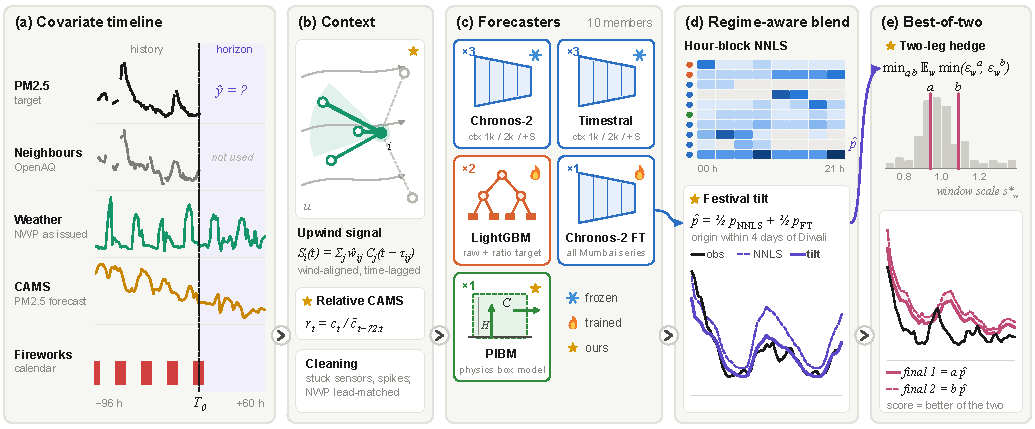
\includegraphics[width=\textwidth]{figures/pipeline_paper.pdf}
  \caption{\textbf{Overview.}
  \textbf{(a)} Inputs around a forecast origin $T_0$ (real series, Byculla, two days after Diwali 2025). Target and
  neighbour PM$_{2.5}$ are read only up to $T_0$; weather forecasts (as issued, lead-matched), the CAMS PM$_{2.5}$
  forecast and the fireworks-night calendar are known over the 84-h horizon.
  \textbf{(b)} The upwind signal $S_i(t)$ averages neighbour concentrations weighted by wind alignment and distance
  and lagged by travel time $\tau_{ij}$; CAMS enters relative to its own 72-h mean, which removes year-to-year drift.
  \textbf{(c)} Ten forecasters: Chronos-2 and Timestral zero-shot with three context variants each, a Chronos-2
  fine-tuned on all Mumbai series, two LightGBM direct multi-horizon models, and PIBM, a physics-informed box model
  (hourly mass balance with emission, mixing height $H$ and ventilation, fitted by backpropagation through time).
  \textbf{(d)} Non-negative least-squares stacking on out-of-fold forecasts with one weight set per 3-h block of
  target hour (heat map; rows are members, coloured by family). For origins within four days after Diwali the
  festival tilt averages the blend with the fine-tuned Chronos-2, removing the blend's post-Diwali over-forecast
  (inset: 2024, two days after Diwali).
  \textbf{(e)} The leaderboard keeps the better of two selected submissions, so the finals are $a\hat p$ and
  $b\hat p$ with $(a,b)$ minimising the expected best-of-two window RMSE; the histogram shows the per-window optimal
  scale $s^*_w$ over 127 backtest windows, and the inset shows a 2025 window where the low leg wins.
  \textcolor[HTML]{D99A00}{$\star$}~marks our contributions.}
  \label{fig:pipeline}
\end{figure*}
% needs \usepackage[table]{xcolor} (or \usepackage{xcolor}) for the coloured star; plain $\star$ also works.
